\begin{figure}
\centering
\begin{tabular}{ccc}
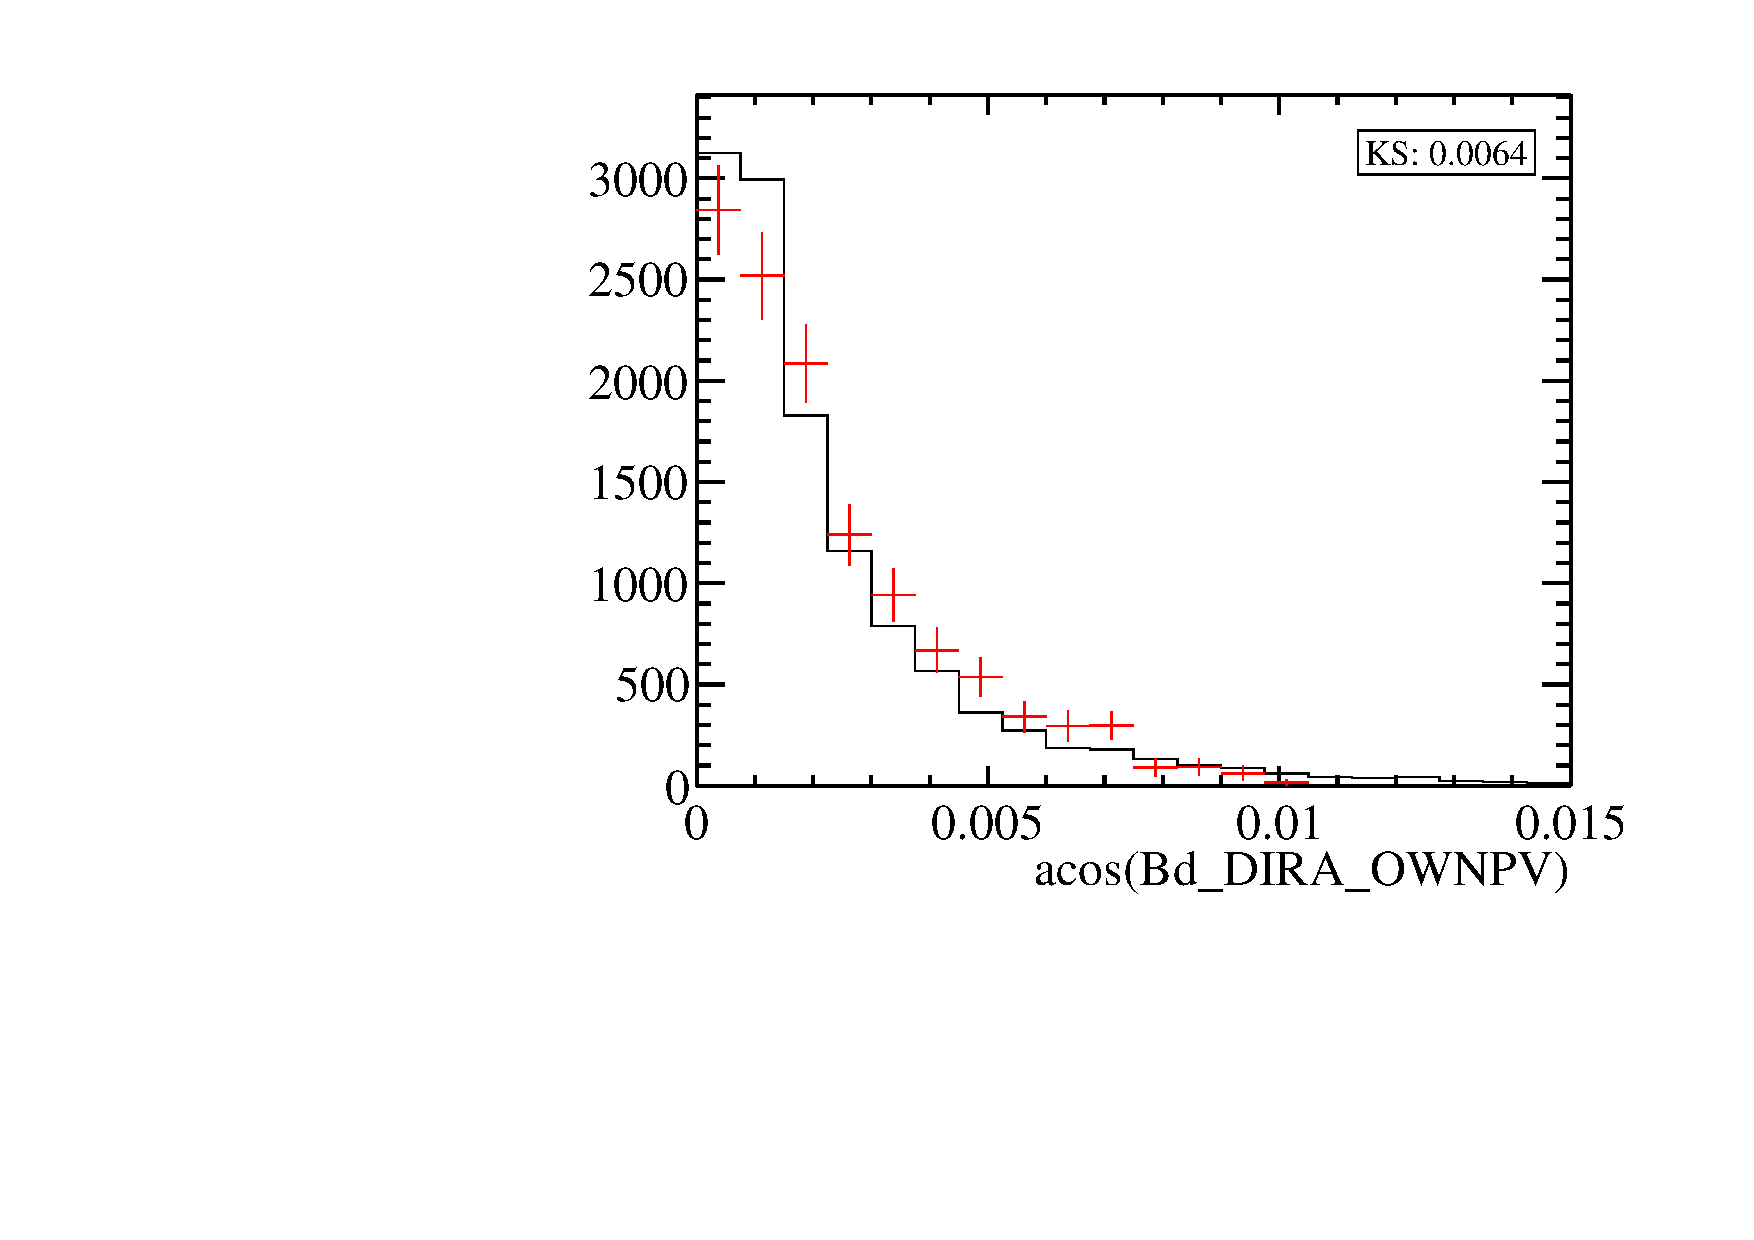
\includegraphics[width=0.3\textwidth]{ANA_resources/Plots/Monte_carlo/data_vs_MC/weight/Kpi/acos(Bd_DIRA_OWNPV)_2016.pdf} & 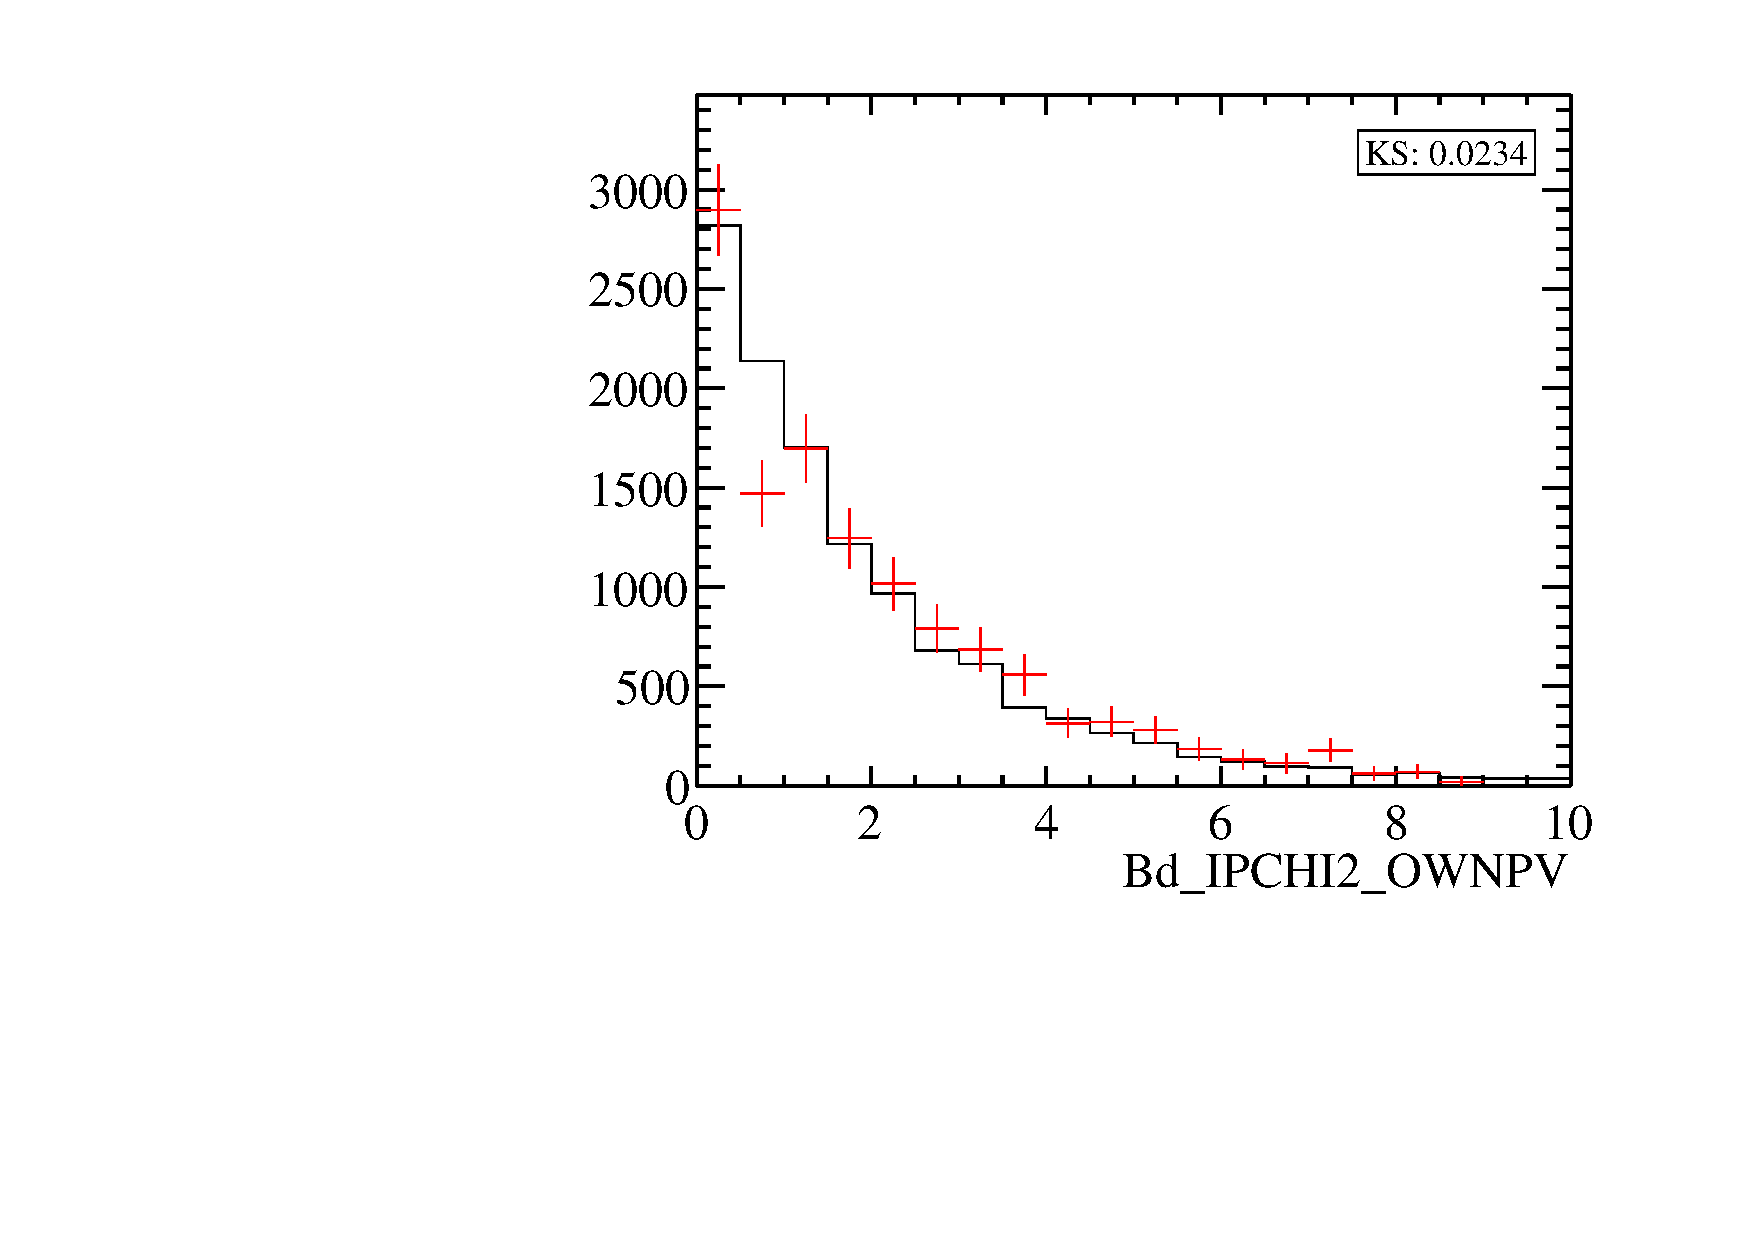
\includegraphics[width=0.3\textwidth]{ANA_resources/Plots/Monte_carlo/data_vs_MC/weight/Kpi/Bd_IPCHI2_OWNPV_2016.pdf} & 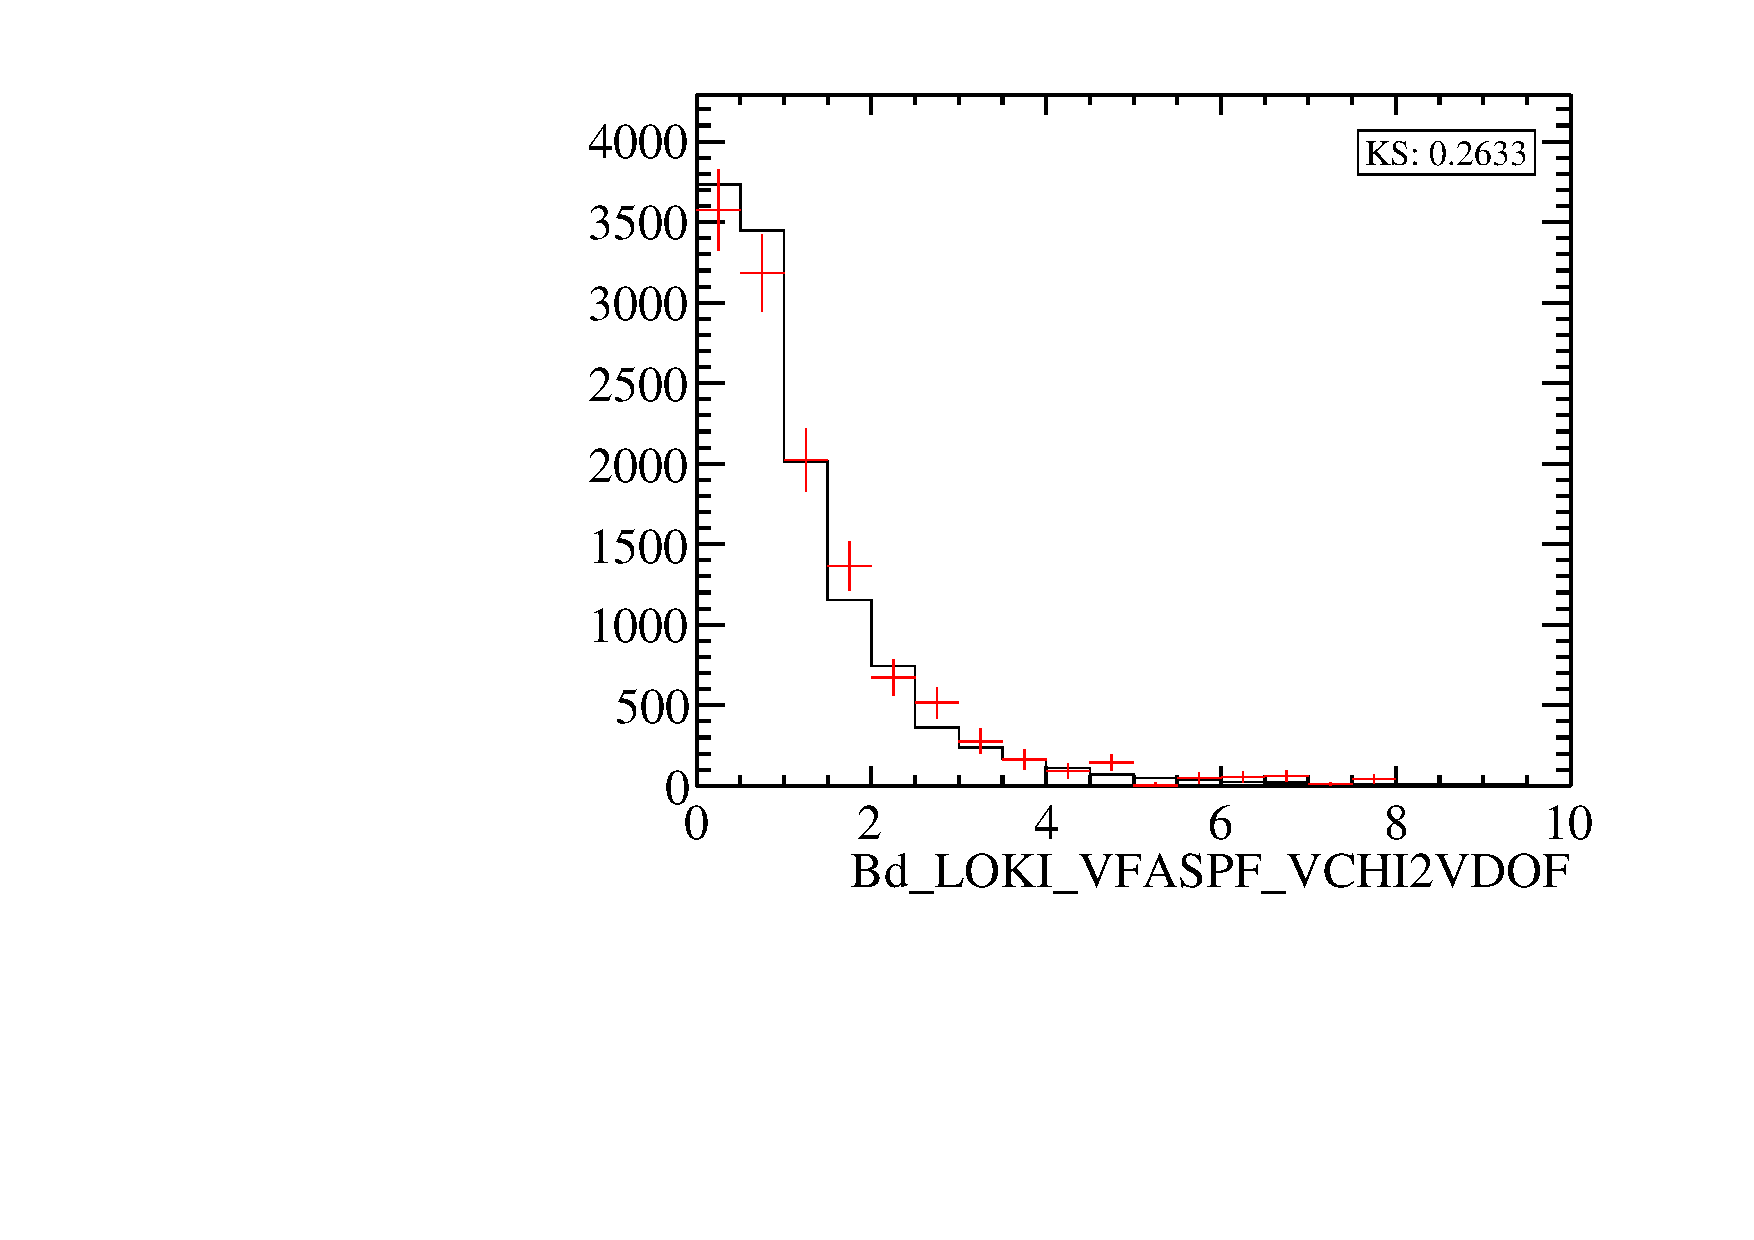
\includegraphics[width=0.3\textwidth]{ANA_resources/Plots/Monte_carlo/data_vs_MC/weight/Kpi/Bd_LOKI_VFASPF_VCHI2VDOF_2016.pdf} \\
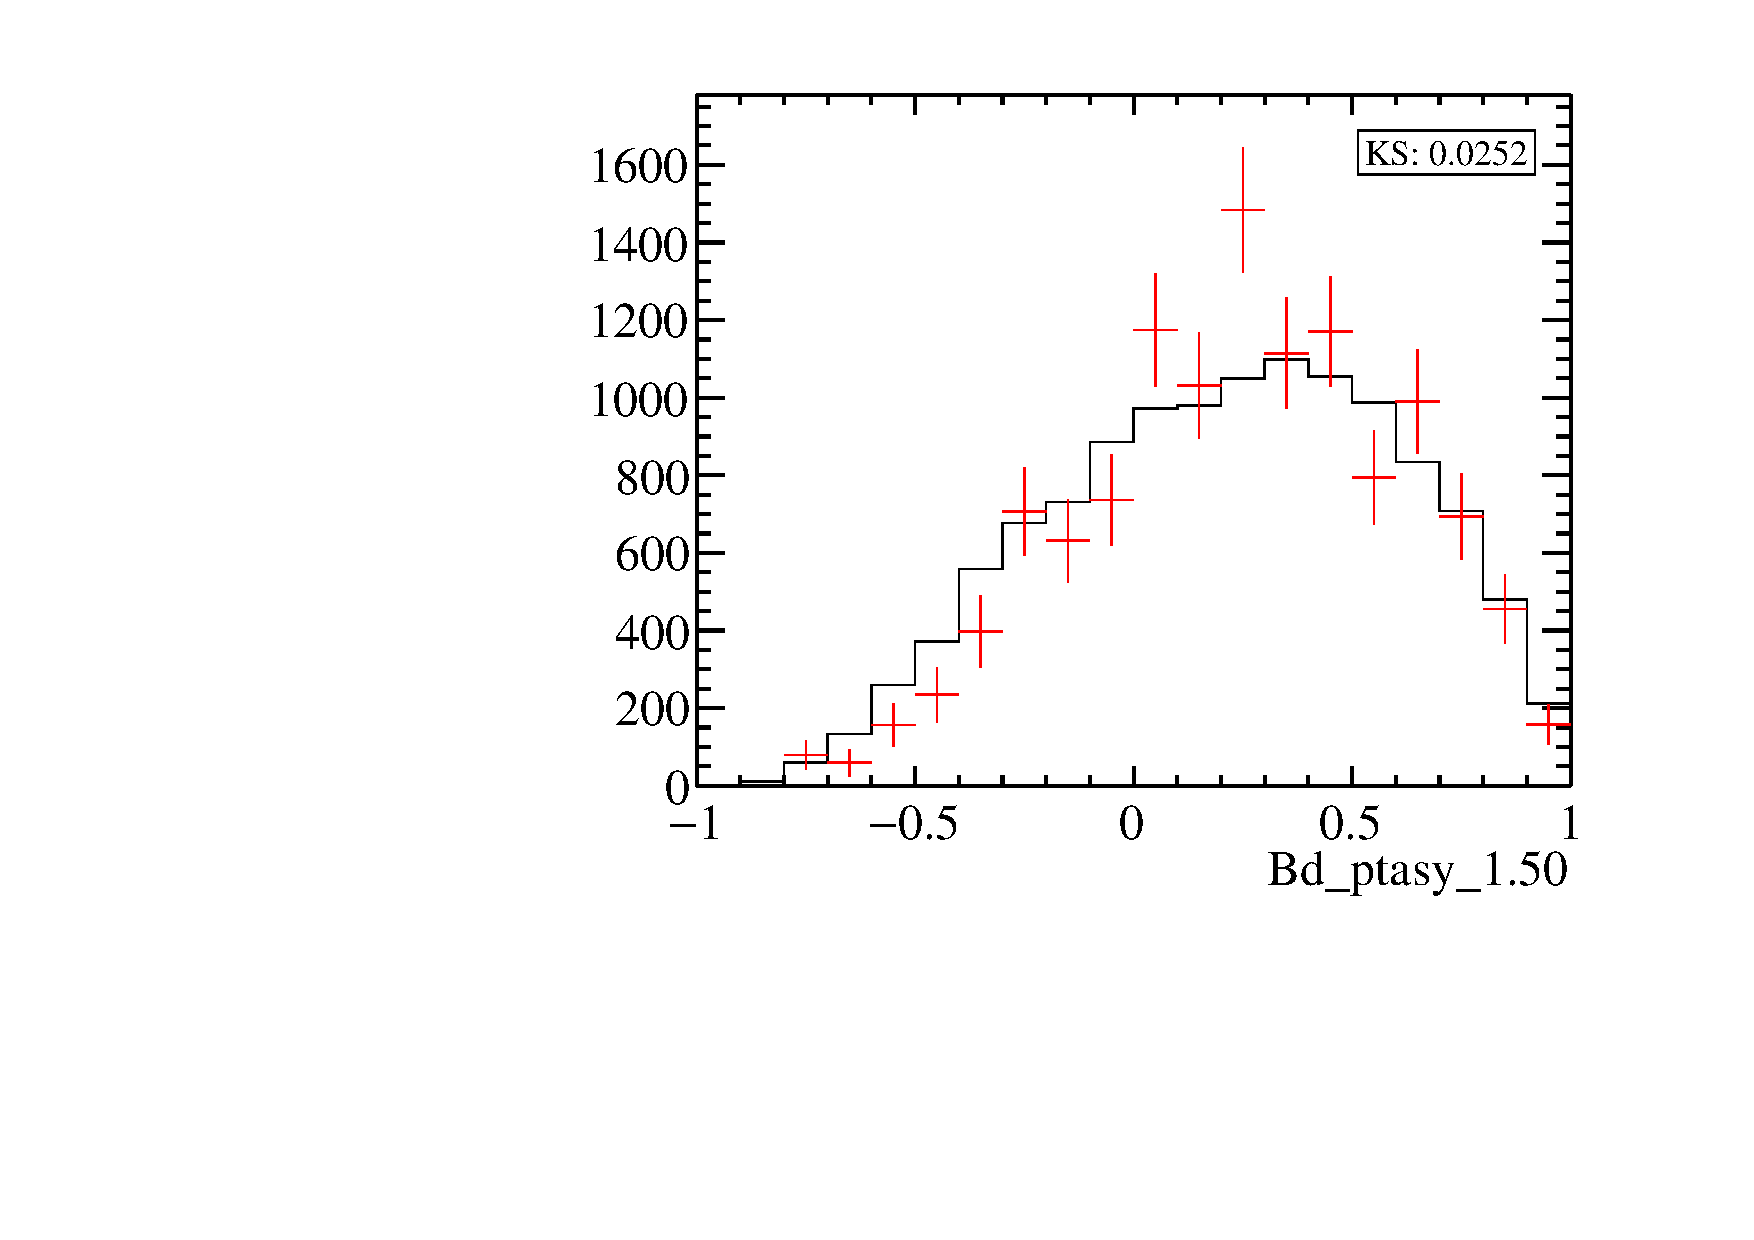
\includegraphics[width=0.3\textwidth]{ANA_resources/Plots/Monte_carlo/data_vs_MC/weight/Kpi/Bd_ptasy_1_50_2016.pdf} & 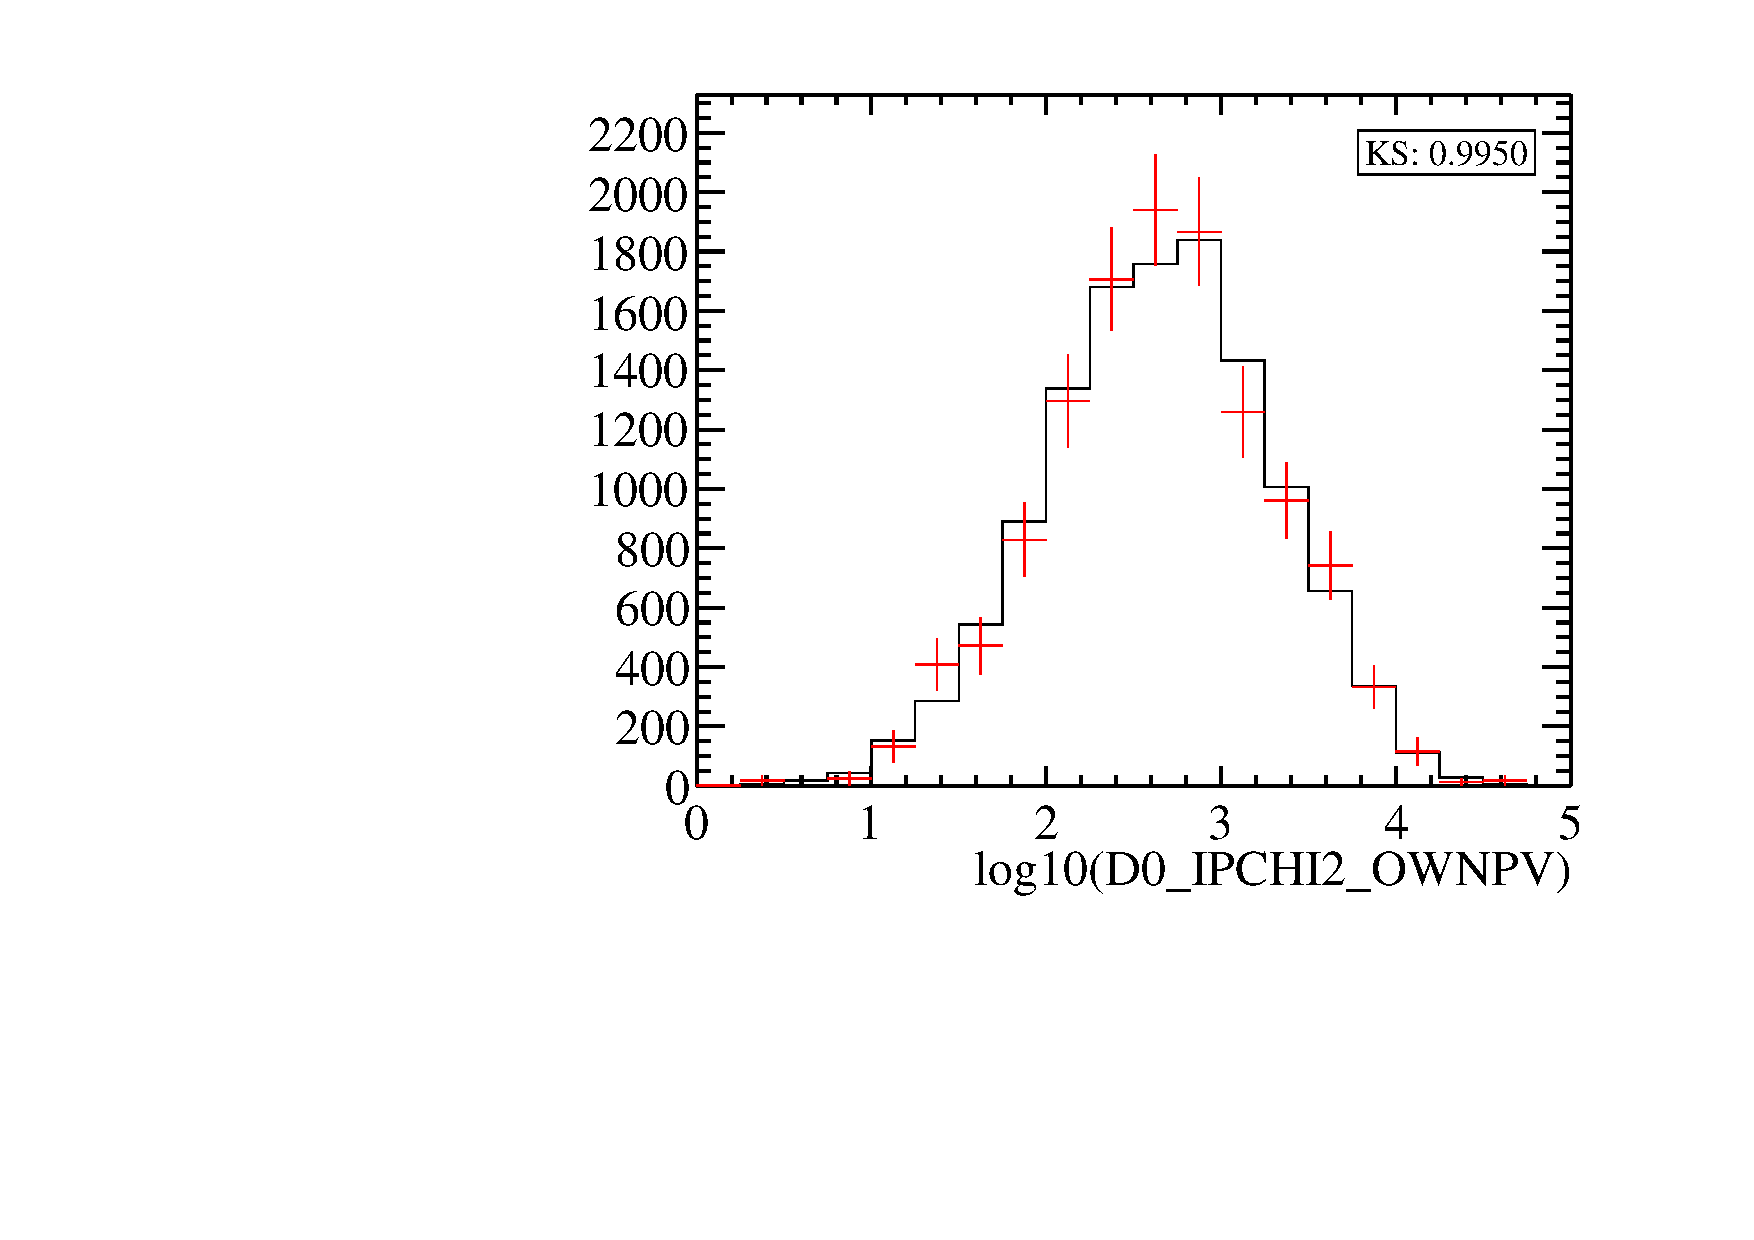
\includegraphics[width=0.3\textwidth]{ANA_resources/Plots/Monte_carlo/data_vs_MC/weight/Kpi/log10(D0_IPCHI2_OWNPV)_2016.pdf} & 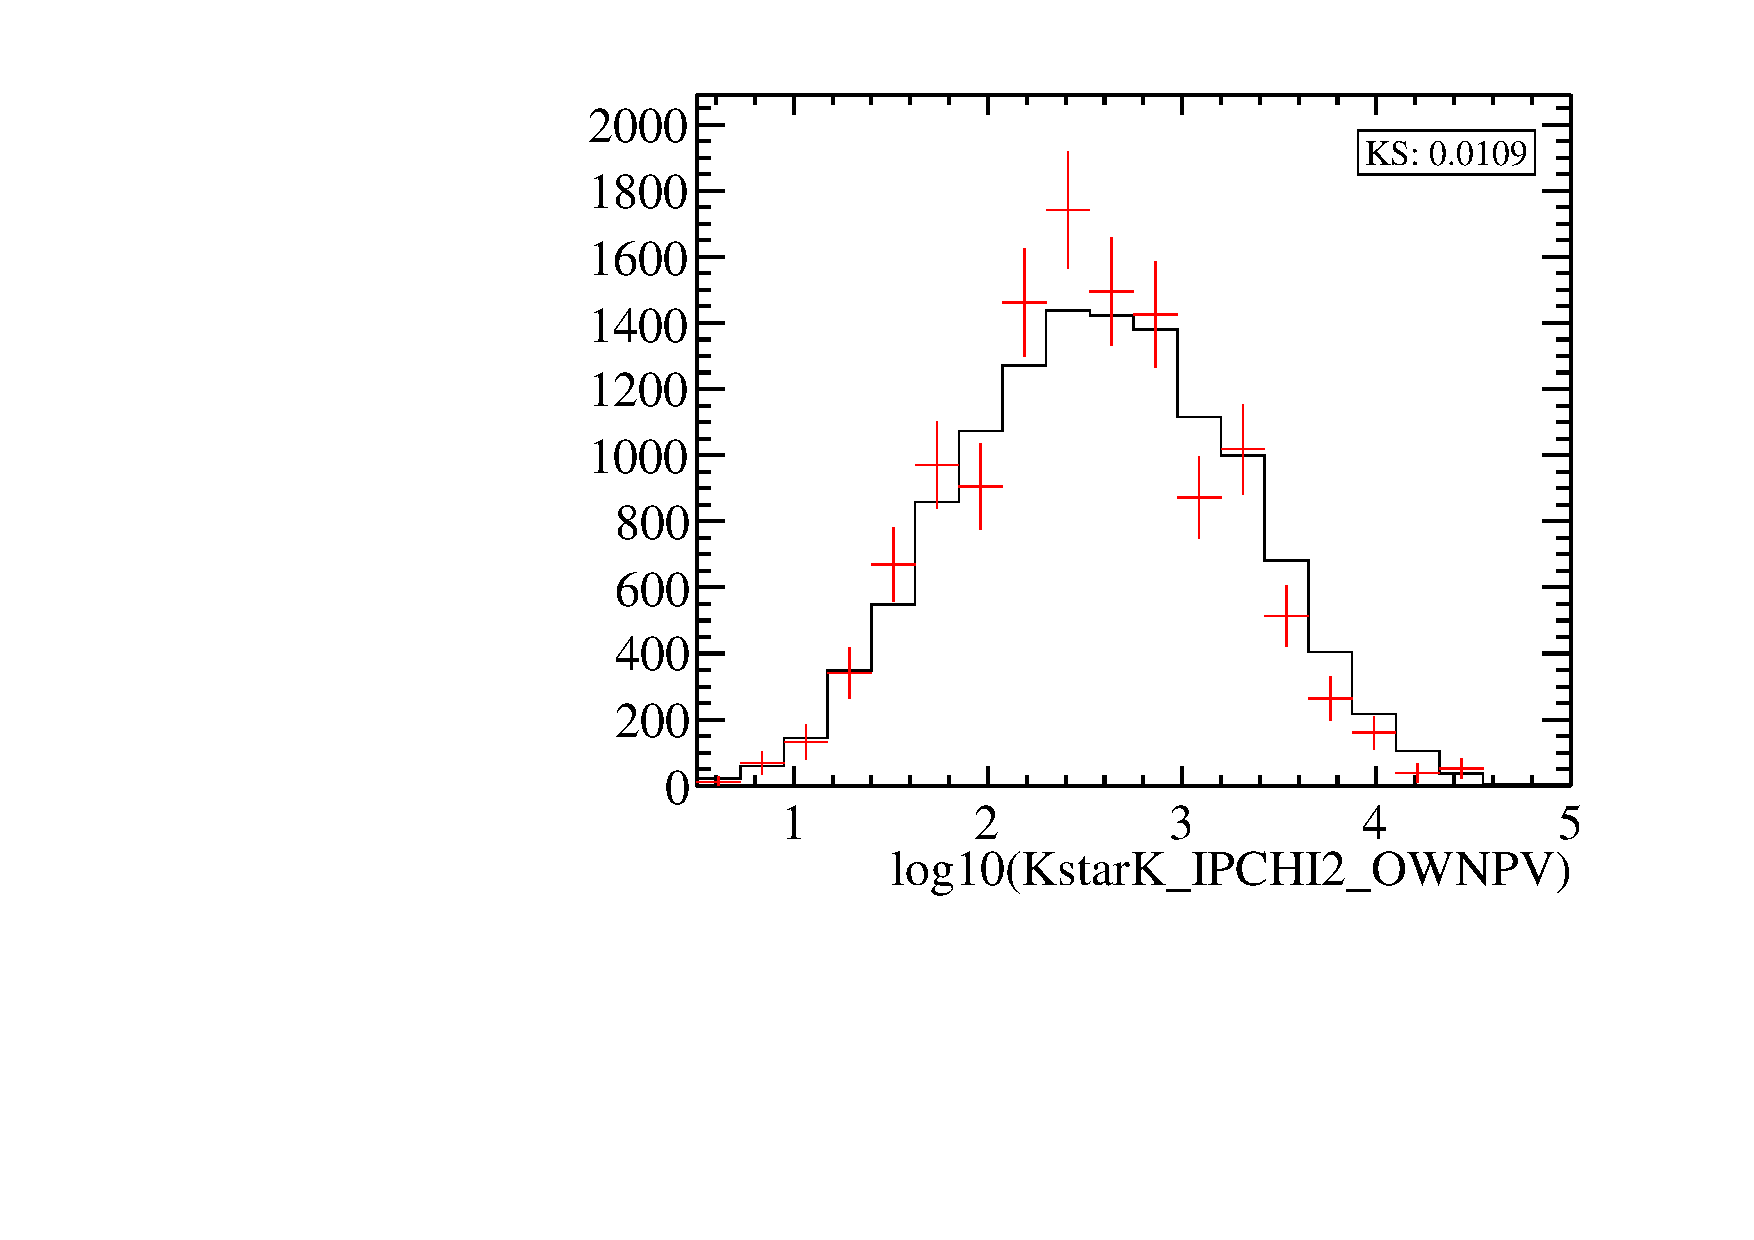
\includegraphics[width=0.3\textwidth]{ANA_resources/Plots/Monte_carlo/data_vs_MC/weight/Kpi/log10(KstarK_IPCHI2_OWNPV)_2016.pdf} \\
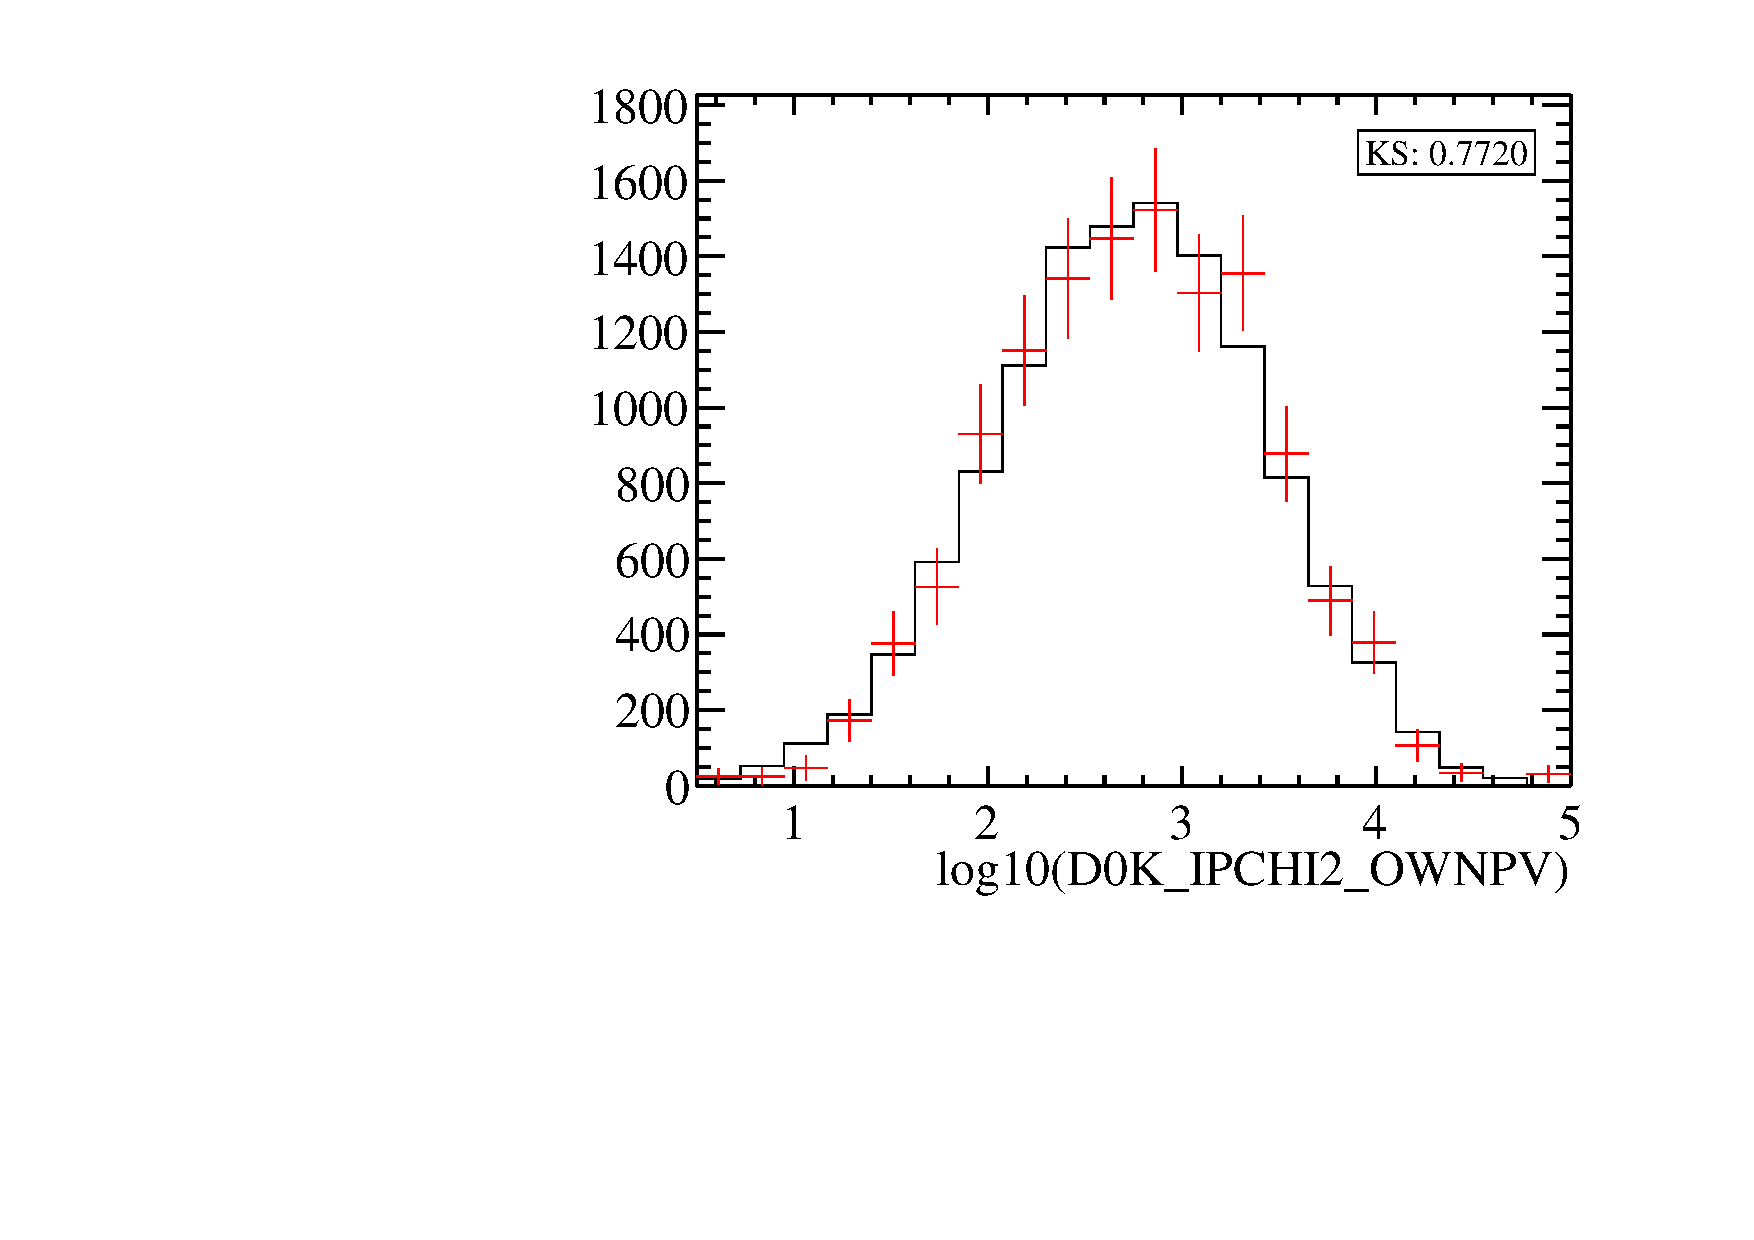
\includegraphics[width=0.3\textwidth]{ANA_resources/Plots/Monte_carlo/data_vs_MC/weight/Kpi/log10(D0K_IPCHI2_OWNPV)_2016.pdf} & 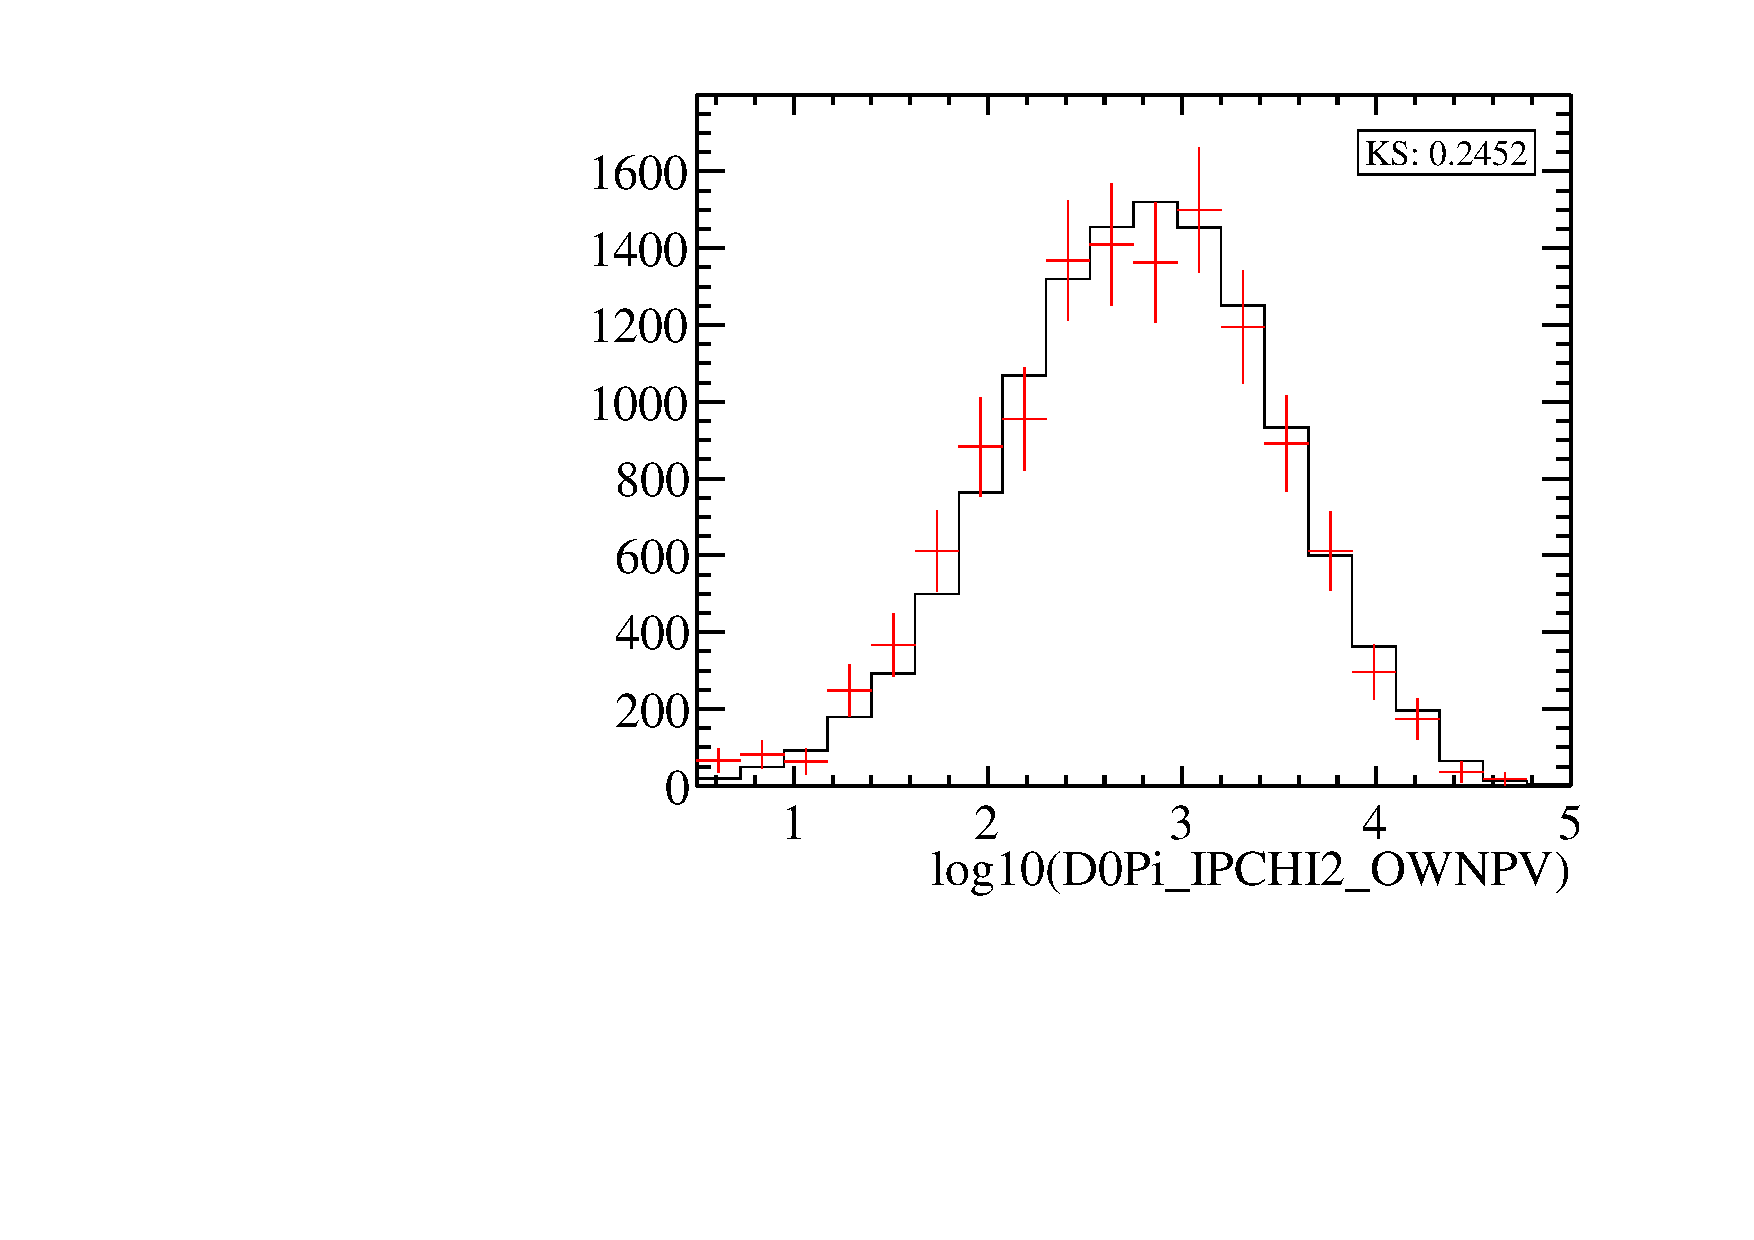
\includegraphics[width=0.3\textwidth]{ANA_resources/Plots/Monte_carlo/data_vs_MC/weight/Kpi/log10(D0Pi_IPCHI2_OWNPV)_2016.pdf} & 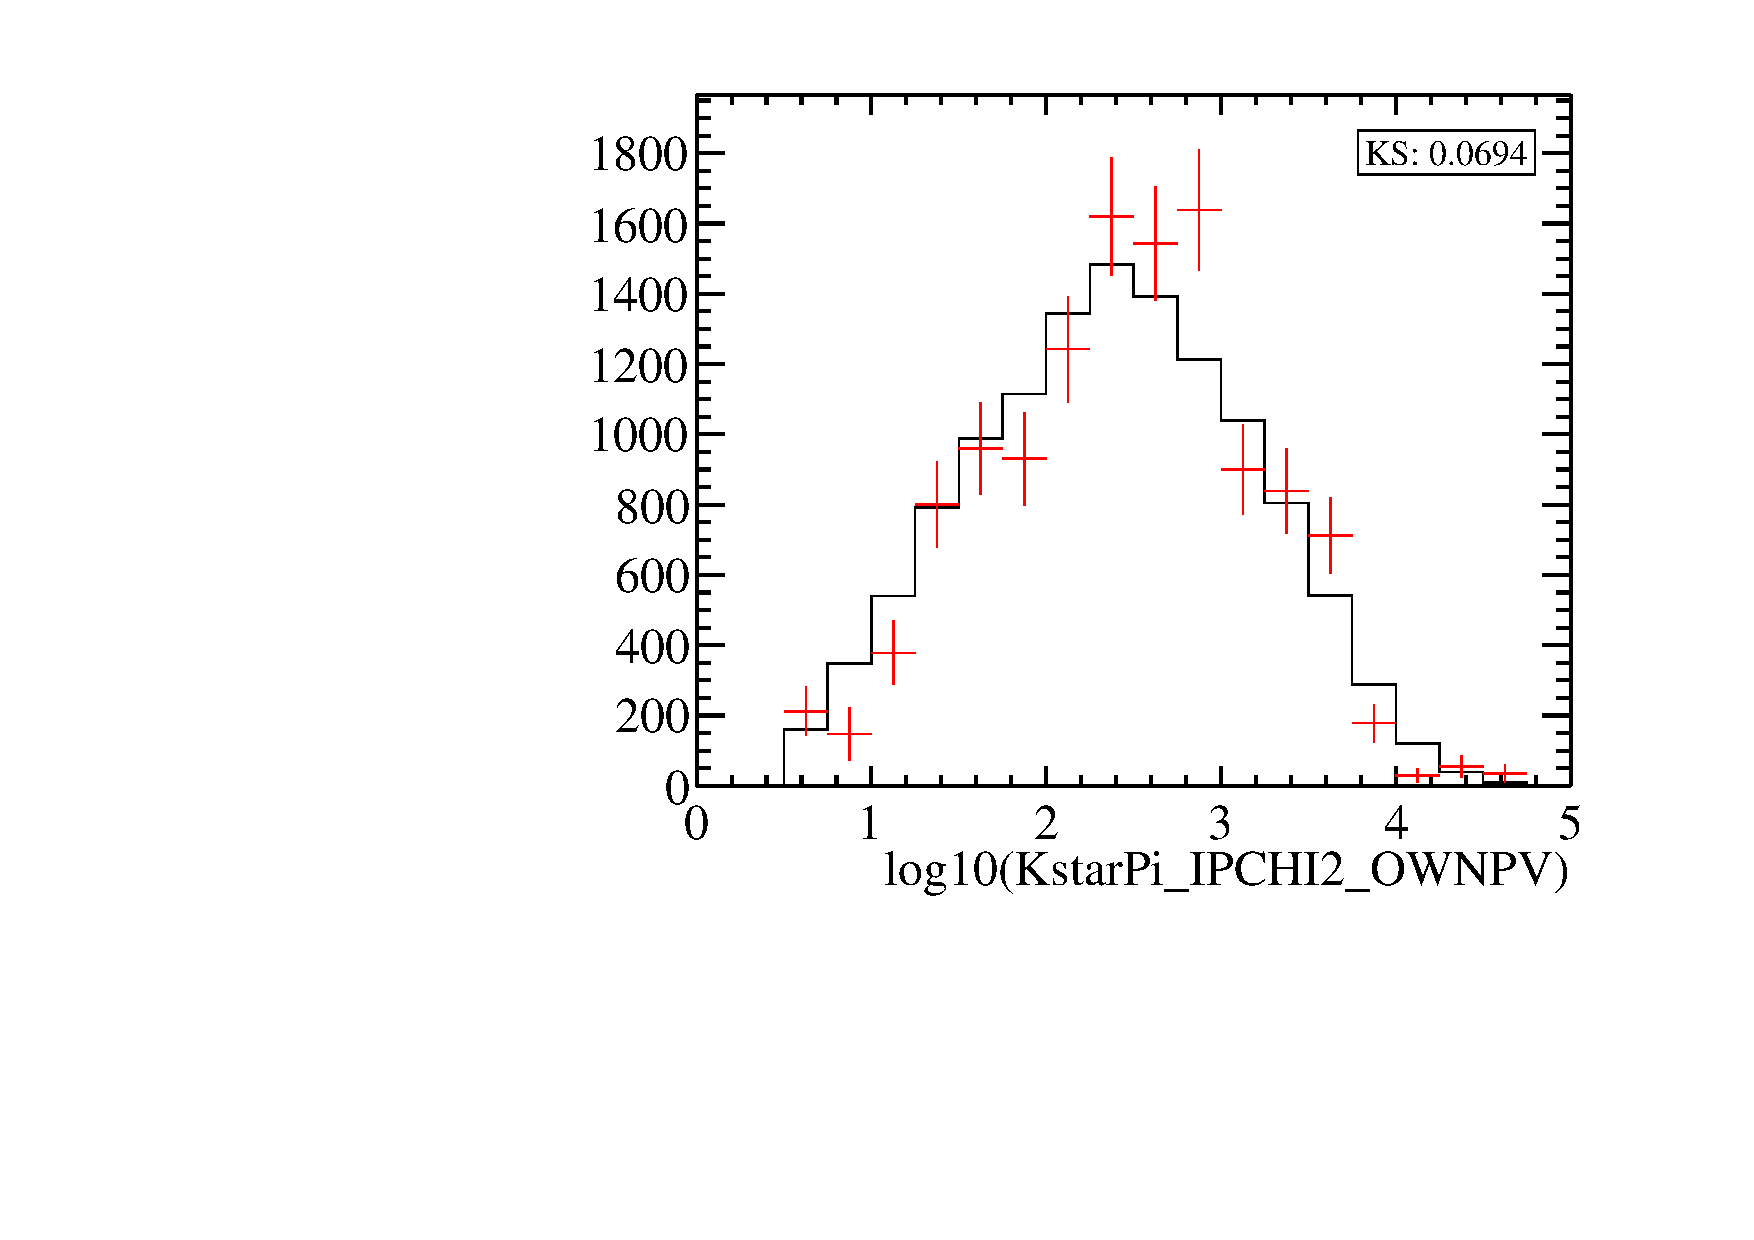
\includegraphics[width=0.3\textwidth]{ANA_resources/Plots/Monte_carlo/data_vs_MC/weight/Kpi/log10(KstarPi_IPCHI2_OWNPV)_2016.pdf} \\
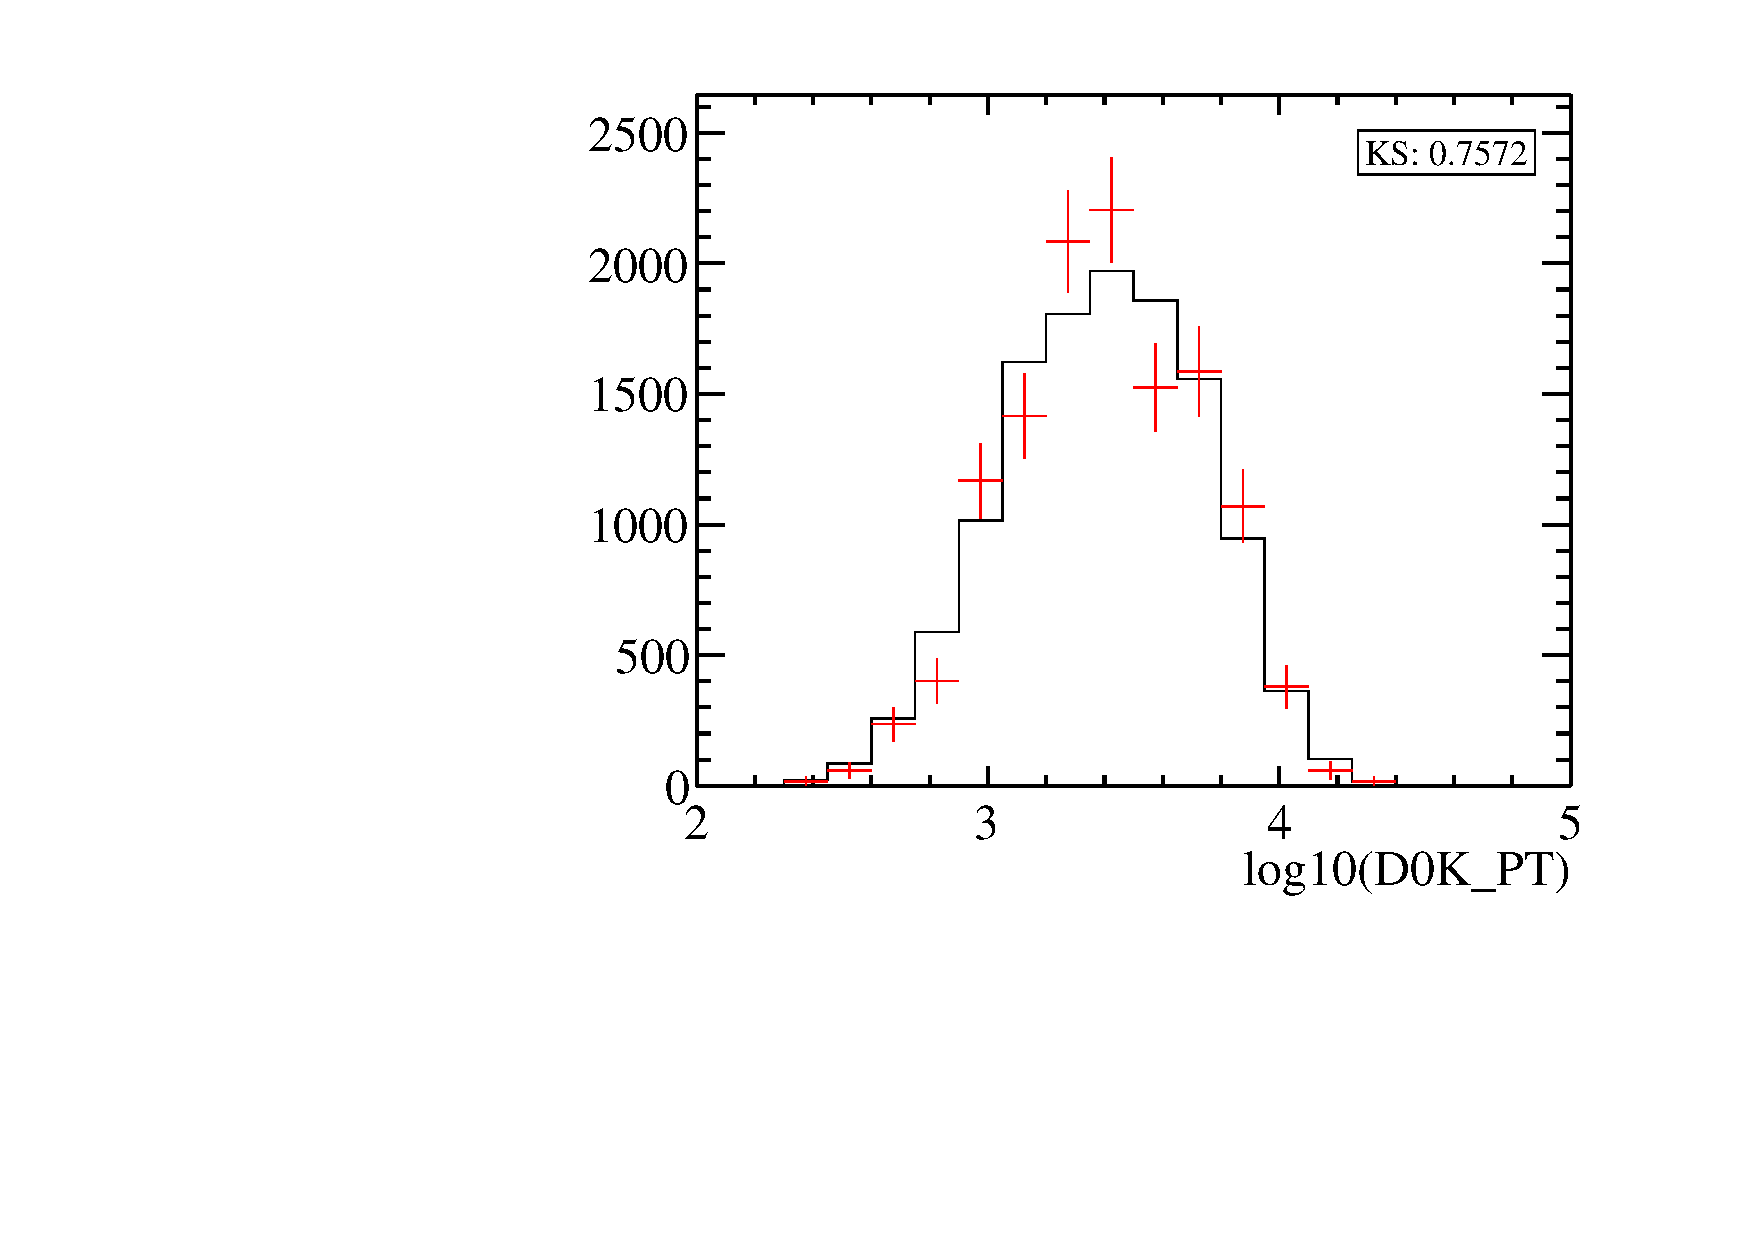
\includegraphics[width=0.3\textwidth]{ANA_resources/Plots/Monte_carlo/data_vs_MC/weight/Kpi/log10(D0K_PT)_2016.pdf} & 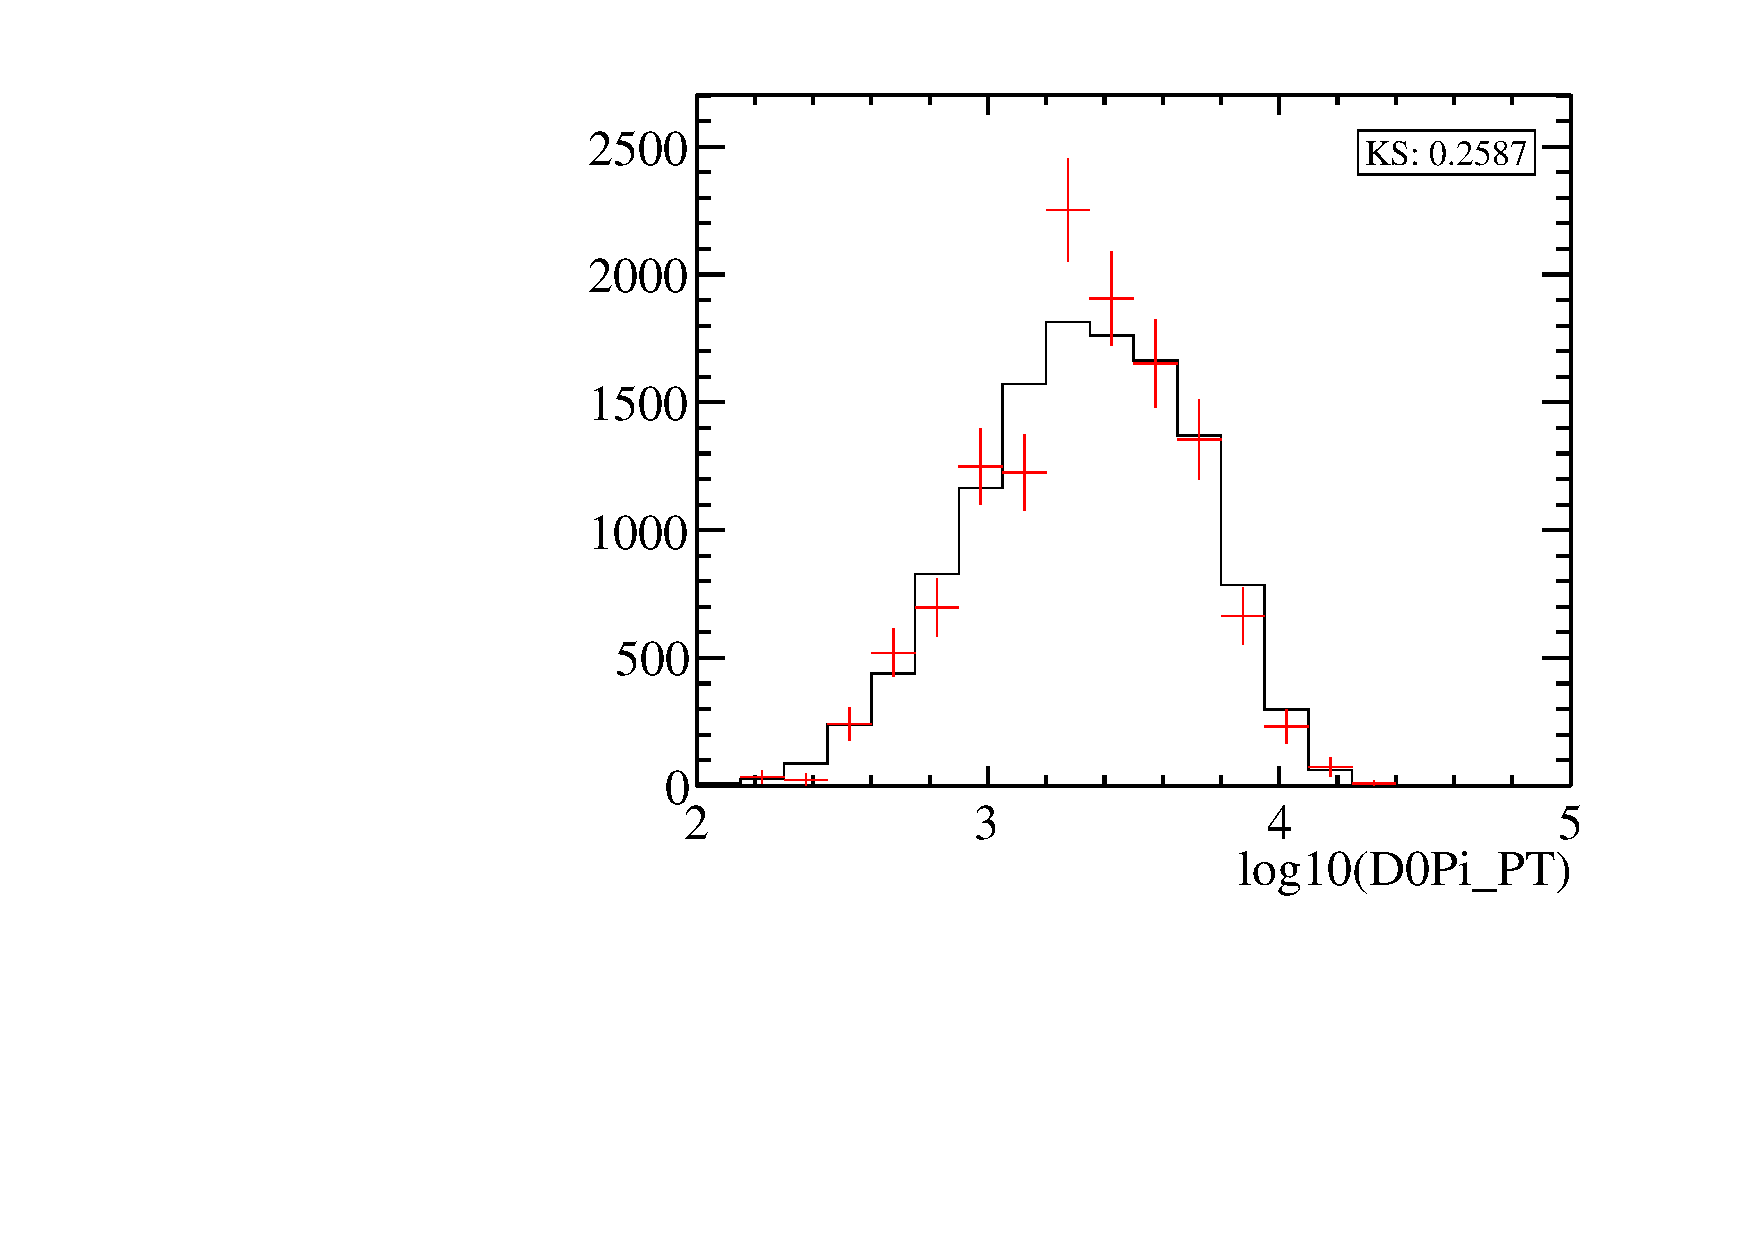
\includegraphics[width=0.3\textwidth]{ANA_resources/Plots/Monte_carlo/data_vs_MC/weight/Kpi/log10(D0Pi_PT)_2016.pdf} & 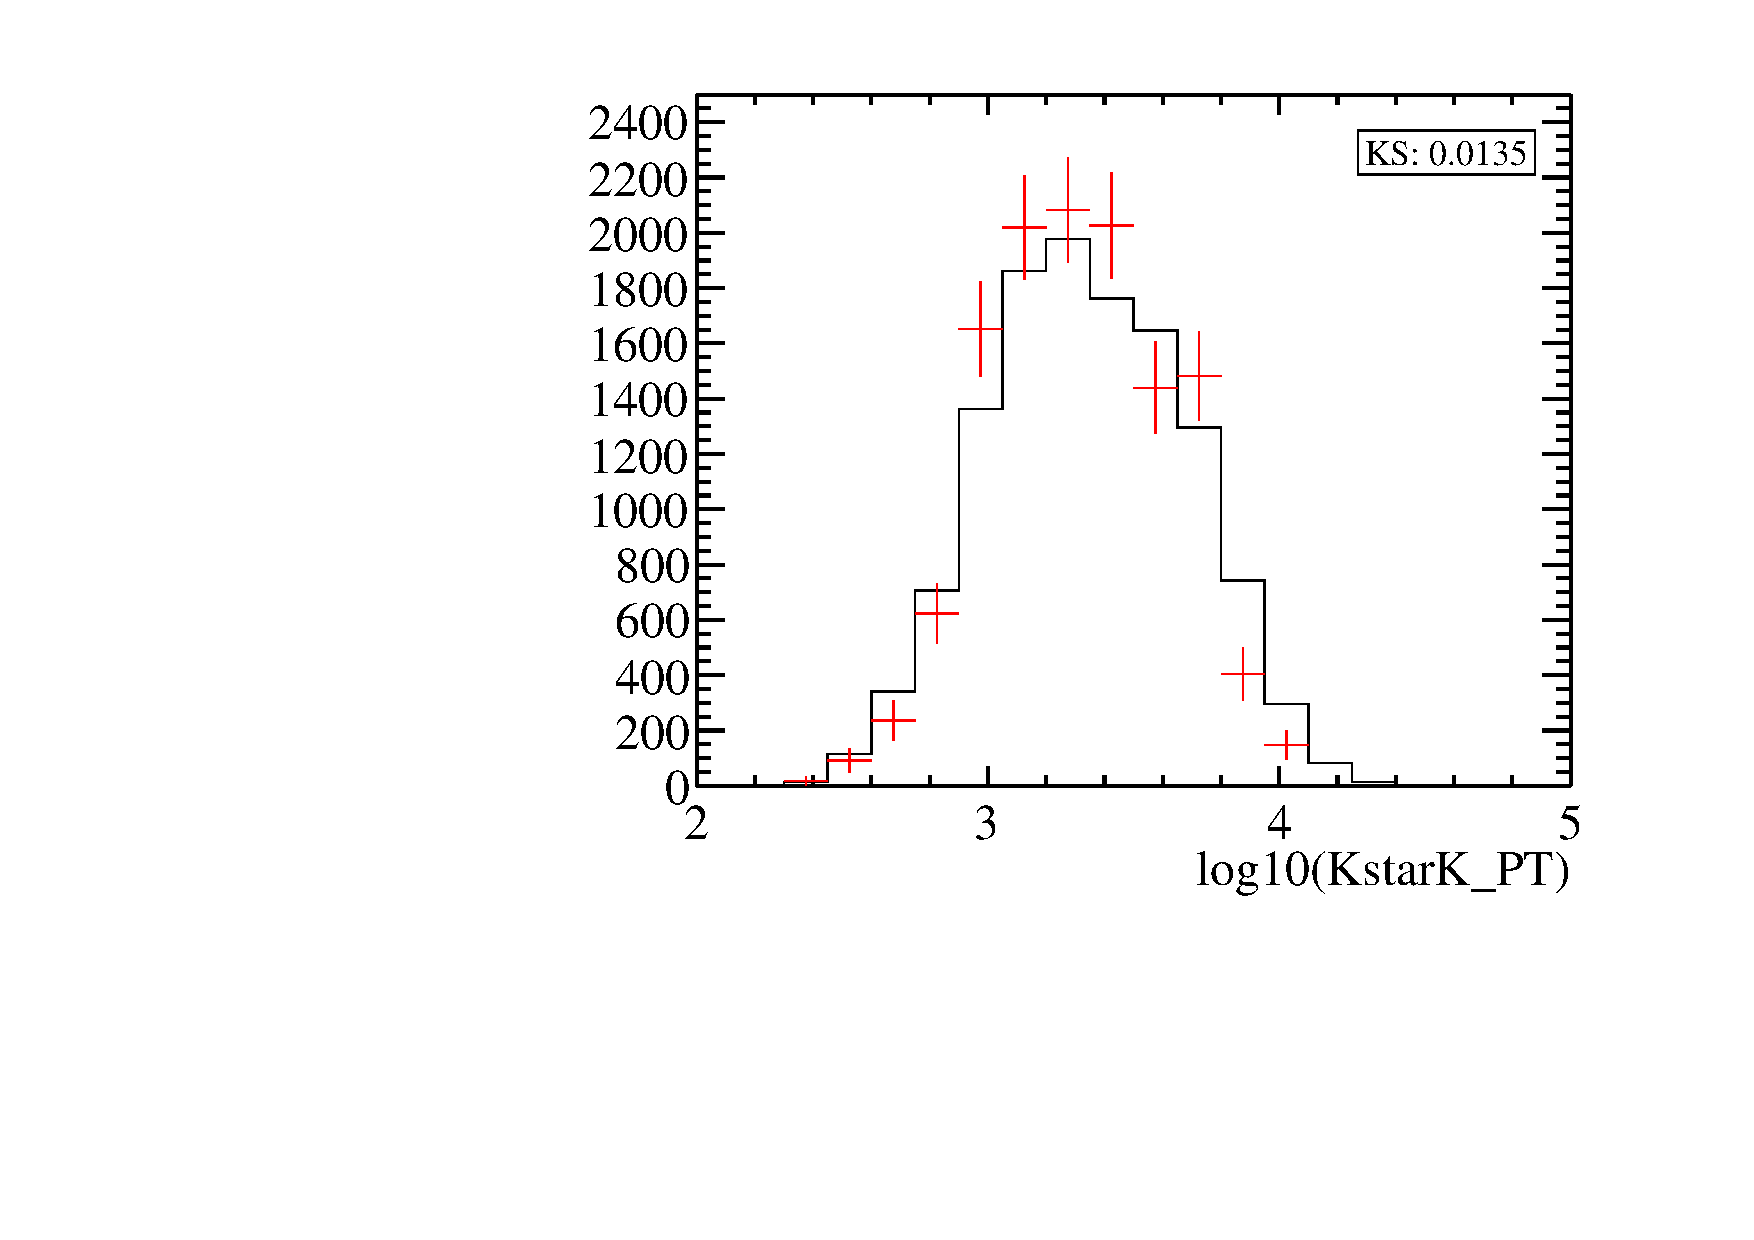
\includegraphics[width=0.3\textwidth]{ANA_resources/Plots/Monte_carlo/data_vs_MC/weight/Kpi/log10(KstarK_PT)_2016.pdf} \\
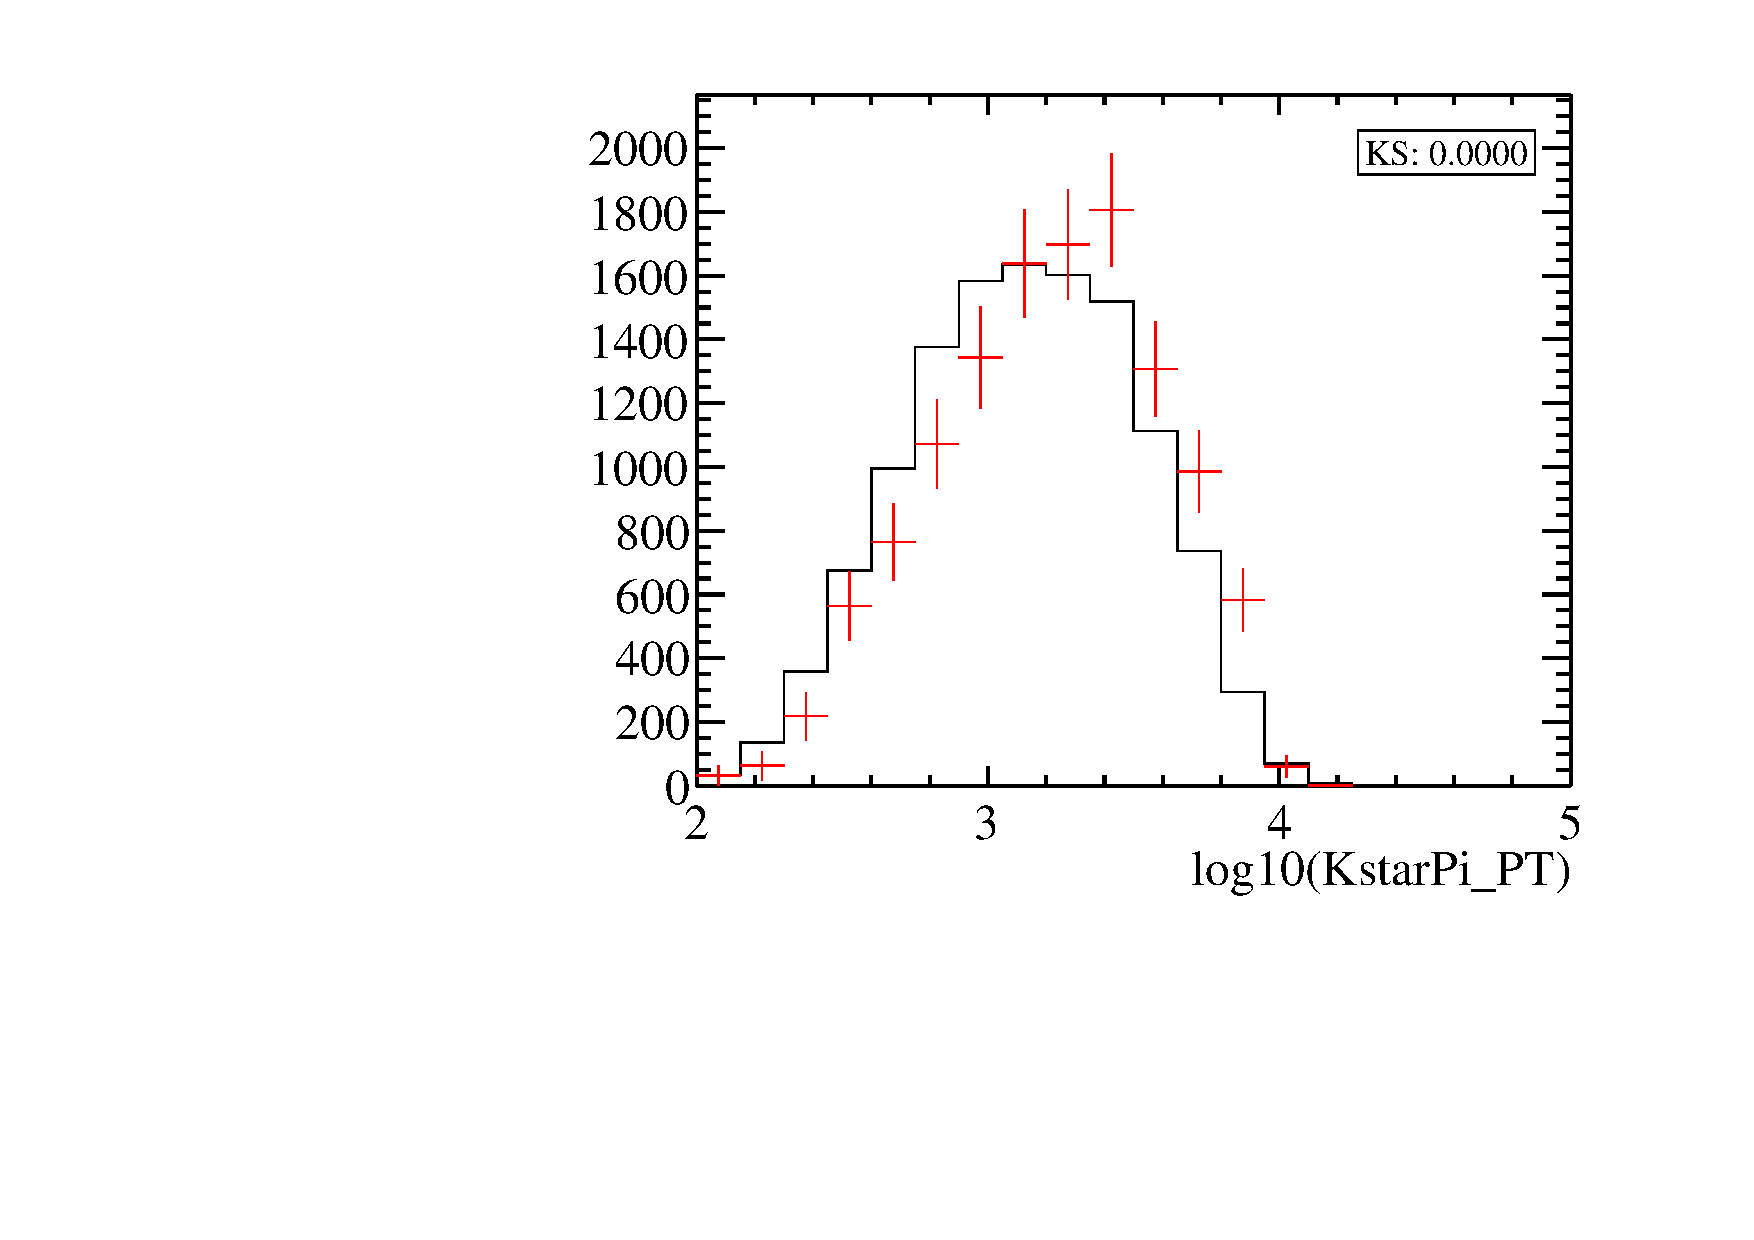
\includegraphics[width=0.3\textwidth]{ANA_resources/Plots/Monte_carlo/data_vs_MC/weight/Kpi/log10(KstarPi_PT)_2016.pdf} & & \\
\end{tabular}
\caption{Comparison of sWeighted 2016 data (red points) and selected, weighted Monte Carlo (black histogram) in the $K\pi$ mode for the variables used in the $K\pi$ BDT, after the MC is reweighted to match the $B^0$ $p_{T}$ and $\eta$ in the data.}
\label{fig:data_vs_MC_Kpi_2016}
\end{figure}
